\documentclass[6008notes.tex]{subfiles}
\begin{document}
\graphicspath{ {images/infgraph/} }

\section{Inference in Graphical Models - Marginalization}

\subsection{Two Fundamental Inference Tasks in Graphical Models}

Now that we have introduced graphical models for representing probability distributions, we proceed to solving problems of inference. As we have seen, observations can be taken care of quite easily and once we account for them, we are left with a new graphical model that is only over the random variables that we don't get to observe, which are called ``hidden'' or ``latent'' random variables. Thus, our discussion to follow will be about graphical models where we don't explicitly mention conditioning, \textit{with the idea that the conditioning has already happened!}

Given a graphical model with graph $G=(V,E)$ and its associated node and edge potentials, the two fundamental inference tasks we focus on are as follows:

\begin{itemize}
\item \textbf{(Marginalization)} Compute marginal probability table $p_{X_ i}$ for every $i \in V$.

\item \textbf{(Most probable configuration)} Compute the most probable configuration $(\widehat{x}_1, \widehat{x}_2, \dots , \widehat{x}_ n)$ such that

{\centering$(\widehat{x}_1, \widehat{x}_2, \dots , \widehat{x}_ n) = \arg \max _{x_1, x_2, \dots , x_ n} p_{X_1, X_2, \dots , X_ n}(x_1, x_2, \dots , x_ n).$ \par}
\end{itemize}
 
Again, we are assuming conditioning has already happened. This means that if we observed random variable $Y=y$ and already accounted for it, then the graphical model that remains is only over random variables $X_1, \dots ,X_n$ and so in the first task above, the table $p_{X_ i}$ actually corresponds to $p_{X_ i \mid Y}(\cdot \mid y)$ and the second task would compute the most probable configuration in the posterior distribution $p_{X_1, \dots , X_ n \mid Y}(\cdots \mid y)$. (Note that there was nothing special about us calling the random variables in a graphical model $X_1, \dots ,X_n$. Doing so was just to make the notation simple, but the random variables could be called whatever you want, including having $X_i$'s and $Y_i$'s, and also observing multiple random variables rather than just observing one random variable is handled the same way: fix the values for what has been observed, which corresponds to removing those nodes from the original graphical model and changing potential tables to account for the observations.)

We now focus on the inference task of marginalization in graphical models.


\subsection{The Sum-Product Algorithm}

\textbf{What about graphical models that aren't tree-structured and that don't have loops?} Think about why in such cases, the different disconnected pieces can be treated separately (and each of these pieces of the graph will be a tree)! For example, when computing the marginal distribution $p_{x_i}$ for a specific node $i$, any node that isn't reachable from $i$ doesn't matter in the computation. So we can always turn the problem into just looking at one tree at a time.

\textbf{Marginalization: A Worked Example}

Let's work through an example of how to marginalize in an undirected graphical model. This example will illustrate a general algorithm for marginalization, which we can write a computer program for.

Suppose random variables $X_1,X_2,X_3,X_4,X_5$ each take on values in the set $\mathcal{X}$ and have the following joint distribution:

\begin{eqnarray*}
p_{X_1, \dots, X_n}(x_1, \dots, x_n)
&=& \frac{1}{Z}\phi_{1}(x_{1})\phi_{2}(x_{2})\phi_{3}(x_{3})\phi_{4}(x_{4})\phi_{5}(x_{5}) \\
&& \;
\cdot \psi_{12}(x_{1},x_{2})\psi_{13}(x_{1},x_{3})\psi_{24}(x_{2},x_{4})\psi_{25}(x_{2},x_{5}).
\end{eqnarray*}

This joint distribution corresponds to the following undirected graphical model:

{\centering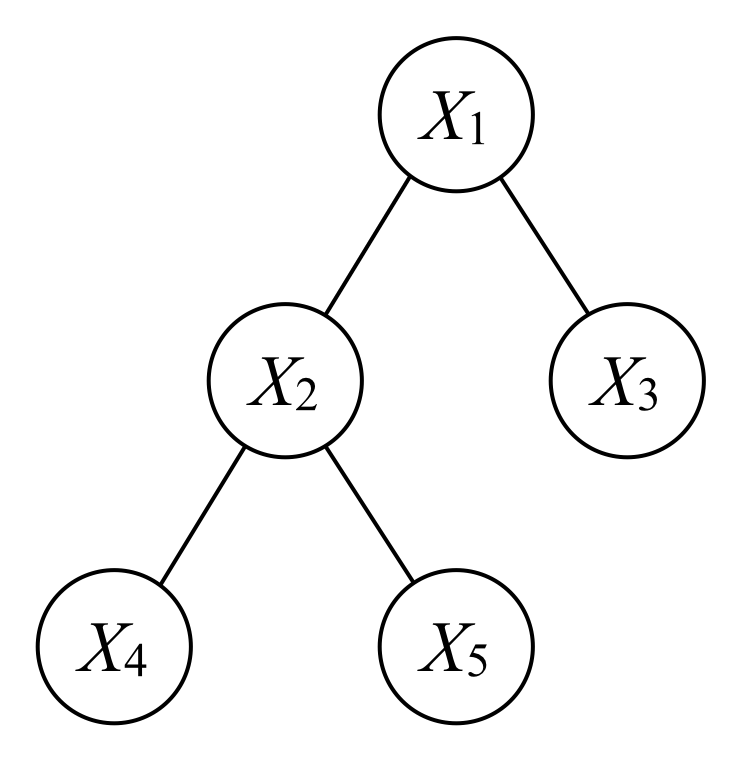
\includegraphics[scale=0.4]{images_sec-graphical-models-five-node-example} \par}

Let's compute the marginal distribution $p_{x_i}$. This distribution is a table assigning a probability to each value of $\mathcal{X}$. We obtain the marginal distribution for $X_1$ by summing out the other random variables:

\begin{eqnarray*}
p_{X_{1}}(x_{1}) & = &\sum_{x_{2}}\sum_{x_{3}}\sum_{x_{4}}\sum_{x_{5}}p_{X_1,\dots,X_n}(x_1,\dots,x_n)\\
& = & \sum_{x_{2}}\sum_{x_{3}}\sum_{x_{4}}\sum_{x_{5}}
\bigg\{\frac{1}{Z}\phi_{1}(x_{1})\phi_{2}(x_{2})\phi_{3}(x_{3})\phi_{4}(x_{4})\phi_{5}(x_{5}) \\
& & \qquad\qquad\qquad\;\;\;\;
\cdot
\psi_{12}(x_{1},x_{2})\psi_{13}(x_{1},x_{3})\psi_{24}(x_{2},x_{4})\psi_{25}(x_{2},x_{5})\bigg\}.
\end{eqnarray*}

To compute the summation on the right-hand side efficiently on a computer, notice that we can push the summations around a bit taking advantage of the distributive property of arithmetic: $ab+ac=a(b+c)$ for any choice of constants $a,b,c$. For example, only two factors depend on $x_5$ (namely $\phi_5$ and $\psi_{25}$) so we can push the summation over $x_5$ inward as follows:

\begin{eqnarray*}
p_{X_{1}}(x_{1}) & = & \sum_{x_{2}}\sum_{x_{3}}\sum_{x_{4}}\sum_{x_{5}}
\bigg\{\frac{1}{Z}\phi_{1}(x_{1})\phi_{2}(x_{2})\phi_{3}(x_{3})\phi_{4}(x_{4})\phi_{5}(x_{5}) \\
& & \qquad\qquad\qquad\;\;\;\;
\cdot \psi_{12}(x_{1},x_{2})\psi_{13}(x_{1},x_{3})\psi_{24}(x_{2},x_{4})\psi_{25}(x_{2},x_{5}) \bigg\} \\
& = & \sum_{x_{2}}\sum_{x_{3}}\sum_{x_{4}}
\bigg\{\frac{1}{Z}\phi_{1}(x_{1})\phi_{2}(x_{2})\phi_{3}(x_{3})\phi_{4}(x_{4}) \\
& & \qquad\qquad\quad\;\;
\cdot \psi_{12}(x_{1},x_{2})\psi_{13}(x_{1},x_{3})\psi_{24}(x_{2},x_{4})\underbrace{\sum_{x_{5}}\phi_{5}(x_{5})\psi_{25}(x_{2},x_{5})}_{\triangleq m_{5 \rightarrow 2}(x_{2})} \bigg\}.
\end{eqnarray*}

Here we have introduced some notation: $m_{5\rightarrow 2}(x_{2})$ is a value we get from summing out (and thus eliminating) $x_5$ where the result depends on $x_2$. Note that $m_{5\rightarrow 2}$ is a table: there is one entry in the table per value of $x_{2}\in \mathcal{X}$. We use the letter ``m'' since we can interpret $m_{5\rightarrow 2}$ as a message that node 5 sends to node 2.

We can keep pushing sums around:

\begin{eqnarray*}
p_{X_{1}}(x_{1}) & = & \sum_{x_{2}}\sum_{x_{3}}
\bigg\{ \frac{1}{Z}\phi_{1}(x_{1})\phi_{2}(x_{2})\phi_{3}(x_{3}) \\
& & \qquad\quad\;\;\;
\cdot \psi_{12}(x_{1},x_{2})\psi_{13}(x_{1},x_{3})m_{5\rightarrow2}(x_{2})\underbrace{\sum_{x_{4}}\phi_{4}(x_{4})\psi_{24}(x_{2},x_{4})}_{\triangleq m_{4\rightarrow2}(x_{2})} \bigg\} \\
 & = & \sum_{x_{2}}\sum_{x_{3}}
\bigg\{ \frac{1}{Z}\phi_{1}(x_{1})\phi_{2}(x_{2})\phi_{3}(x_{3}) \\
& & \qquad\quad\;\;\;
\cdot \psi_{12}(x_{1},x_{2})\psi_{13}(x_{1},x_{3})m_{4\rightarrow2}(x_{2})m_{5\rightarrow2}(x_{2}) \bigg\} \\
 & = & \sum_{x_{2}}\bigg\{ \frac{1}{Z}\phi_{1}(x_{1})\phi_{2}(x_{2})\psi_{12}(x_{1},x_{2}) \\
& & \qquad\;
\cdot m_{4\rightarrow2}(x_{2})m_{5\rightarrow2}(x_{2})\underbrace{\sum_{x_{3}}\phi_{3}(x_{3})\psi_{13}(x_{1},x_{3})}_{\triangleq m_{3\rightarrow1}(x_{1})} \bigg\} \\
 & = & \frac{1}{Z}\phi_{1}(x_{1})m_{3\rightarrow1}(x_{1})\underbrace{\sum_{x_{2}}\phi_{2}(x_{2})\psi_{12}(x_{1},x_{2})m_{4\rightarrow2}(x_{2})m_{5\rightarrow2}(x_{2})}_{\triangleq m_{2\rightarrow1}(x_{1})}\\
 & = & \frac{1}{Z}\underbrace{\phi_{1}(x_{1})m_{2\rightarrow1}(x_{1})m_{3\rightarrow1}(x_{1})}_{\triangleq\widetilde{p}_{X_{1}}(x_{1})},
\end{eqnarray*}

where in the last line, we define $\widetilde{p}_{X_{1}}(\cdot )$ to be a table that just corresponds to an unnormalized version of the marginal distribution of $X_1$. We can readily compute the normalization constant:

{\centering$Z = \sum_{x_{1}}\widetilde{p}_{X_{1}}(x_{1})$ \par}

Once we have computed this, we know the marginal distribution $p_{X_1}$ for $X_1$.

\textbf{Computing Another Marginal Distribution in the Graph}

Now suppose that we want the marginal distribution $p_{X_3}$ for $X_3$. We can approach solving this problem the same way as how we computed the marginal distribution $p_{X_1}$ for $X_1$. But something nice happens, assuming that we've already computed the intermediate tables that we computed to obtain the marginal for $X_1$. In particular, we have

\begin{eqnarray*}
p_{X_{3}}(x_{3}) & = & \sum_{x_{1}}\sum_{x_{2}}\sum_{x_{4}}\sum_{x_{5}}
\bigg\{ \frac{1}{Z}\phi_{1}(x_{1})\phi_{2}(x_{2})\phi_{3}(x_{3})\phi_{4}(x_{4})\phi_{5}(x_{5}) \\
&&\qquad\qquad\qquad\;\;\;\;
\cdot \psi_{12}(x_{1},x_{2})\psi_{13}(x_{1},x_{3})\psi_{24}(x_{2},x_{4})\psi_{25}(x_{2},x_{5}) \bigg\} \\
 & = & \sum_{x_{1}}\sum_{x_{2}}\sum_{x_{4}}
\bigg\{ \frac{1}{Z}\phi_{1}(x_{1})\phi_{2}(x_{2})\phi_{3}(x_{3})\phi_{4}(x_{4})\\
&&\qquad\qquad\quad\;\;
\cdot \psi_{12}(x_{1},x_{2})\psi_{13}(x_{1},x_{3})\psi_{24}(x_{2},x_{4})\underbrace{\sum_{x_{5}}\phi_{5}(x_{5})\psi_{25}(x_{2},x_{5})}_{m_{5\rightarrow2}(x_{2})\text{ - we already computed this}} \bigg\} \\
 & = & \sum_{x_{1}}\sum_{x_{2}}
\bigg\{ \frac{1}{Z}\phi_{1}(x_{1})\phi_{2}(x_{2})\phi_{3}(x_{3}) \\
&&\qquad\qquad
\cdot \psi_{12}(x_{1},x_{2})\psi_{13}(x_{1},x_{3})m_{5\rightarrow2}(x_{2})\underbrace{\sum_{x_{4}}\phi_{4}(x_{4})\psi_{24}(x_{2},x_{4})}_{m_{4\rightarrow2}(x_{2})\text{ - also already computed}} \bigg\} \\
 & = & \sum_{x_{1}}
\bigg\{ \frac{1}{Z}\phi_{1}(x_{1})\phi_{3}(x_{3}) \\
&&\qquad\;
\cdot \psi_{13}(x_{1},x_{3})\underbrace{\sum_{x_{2}}\phi_{2}(x_{2})\psi_{12}(x_{1},x_{2})m_{4\rightarrow2}(x_{2})m_{5\rightarrow2}(x_{2})}_{m_{2\rightarrow1}(x_{1})\text{ - already computed}} \bigg\} \\
 & = & \frac{1}{Z}\phi_{3}(x_{3})\underbrace{\sum_{x_{1}}\phi_{1}(x_{1})\psi_{13}(x_{1},x_{3})m_{2\rightarrow1}(x_{1})}_{\triangleq m_{1\rightarrow3}(x_{3})}\\
 & = & \frac{1}{Z}\underbrace{\phi_{3}(x_{3})m_{1\rightarrow3}(x_{3})}_{\triangleq\widetilde{p}_{X_{3}}(x_{3})}.
\end{eqnarray*}

\textbf{The General Case: The Sum-Product Algorithm}

We are now ready to state the general algorithm for computing marginal distributions for every node in an undirected graphical model. This algorithm specifically works when the corresponding graph is a tree, which means that it has no loops and we can reach from any node in the graph to any other node by traversing along edges. The resulting general algorithm for marginalization is called the \textit{sum-product algorithm} (and popularly also goes by the name \textit{belief propagation}):

\begin{itemize}
\item 1. Choose a root note (arbitrarily) and identify corresponding leaf nodes.
(In our earlier example, we choose node 1 as the root node; the leaf nodes then are nodes 3, 4, and 5.)

\item 2. Proceed from the leaf nodes to the root node computing required messages along the way.
(In our earlier example, we computed messages in the order $m_{5\rightarrow 2}$, $m_{4\rightarrow 2}$, $m_{3\rightarrow 1}$, and $m_{2\rightarrow 1}$.)

When the root node is reached, reverse direction and calculate messages that go back to the leaf nodes
(In our earlier example, we then computed messages $m_{1\rightarrow 3}$ followed by $m_{1\rightarrow 2}$; to further get the marginals at $X_4$ and $X_5$ compute $m_{2\rightarrow 4}$ and $m_{2\rightarrow 5}$.)

The equation for computing the table of messages is given by

{\centering$m_{i\rightarrow j}(x_{j})=\sum _{x_{i}}\bigg[\phi _{i}(x_{i})\psi _{i,j}(x_{i},x_{j})\prod _{k\in \mathcal{N}(i)\text { such that }k\ne j}m_{k\rightarrow i}(x_{i})\bigg],$ \par}
 
where $\mathcal{N}(i)$ denotes the neighboring nodes of node $i$ in the graph.

\item 3. For each node $i$, use the incoming messages to compute the marginal distribution $p_{X_i}$:

{\centering$p_{X_{i}}(x_{i})=\frac{1}{Z}\underbrace{\phi _{i}(x_{i})\prod _{j\in \mathcal{N}(i)}m_{j\rightarrow i}(x_{i})}_{\widetilde{p}_{X_{i}}(x_{i})}.$ \par}
 
Typically, this marginal is computed by first computing the unnormalized table $\widetilde{p}_{X_{i}}$ and then normalizing it; the normalization constant $Z$ is not saved (although it could be).
\end{itemize}


\subsection{Speeding Up Sum-Product}

The sum-product algorithm naively implemented can take time that is more than linear in the number of nodes $n$. We can see this from the worst-case star graph:

{\centering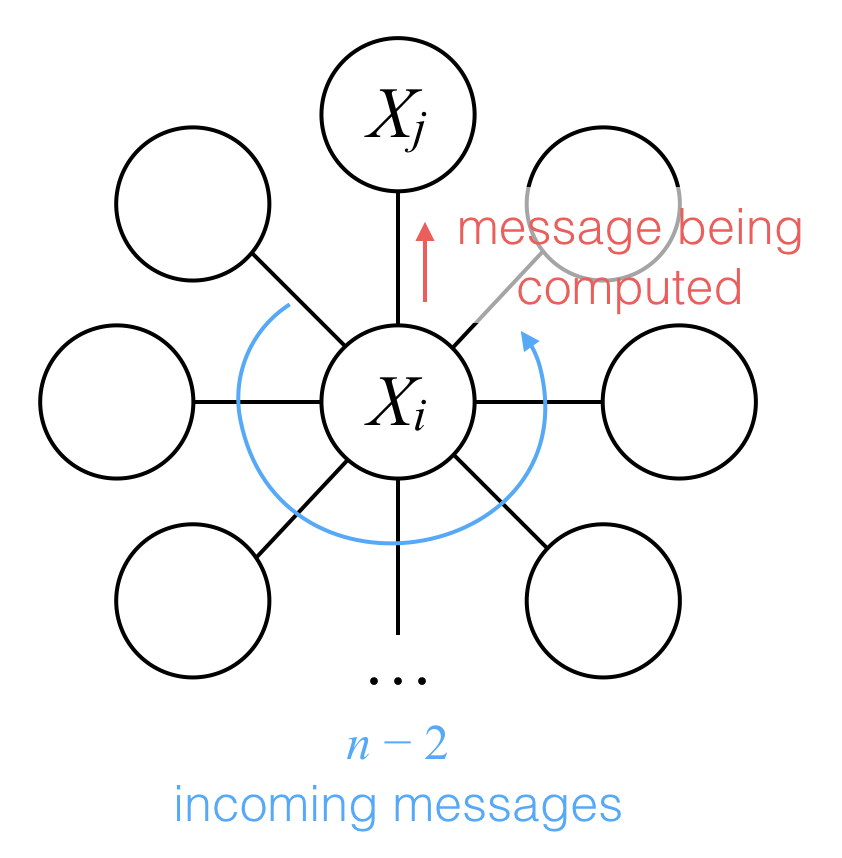
\includegraphics[scale=0.4]{images_ex-sum-product-complexity-star-graph} \par}

In particular with node $i$ referring to the center of the star graph, for every possible node $j$ that is not $i$ (there are $\mathcal{O}(n)$ choices for $j$), the computation of $m_{i\rightarrow j}$ requires taking the product of $\mathcal{O}(n)$ terms, so we get hit by a total running time that at least scales with $n^2$.

It turns out that with clever implementation, we can cut this running time down to linear in $n$. We walk through a way of doing this, which will treat the two passes of the sum-product slightly differently in terms of calculation. Note that this way of speeding up the calculation will require that the message tables always have strictly positive entries. There are ways around this assumption that still keeps the computation linear in $n$ but to keep the exposition here simple we'll stick to strictly positive message table entries.

In what follows, let $d_i$ denote the number of neighbors that node $i$ has; in graph theory, $d_i$ is called the degree of node $i$. As before, assume that every $X_i$ takes on one of $k$ possible values (note that even if the different $X_i$'s took on a different number of values, we can take $k$ to be the maximum alphabet size of any of the $X_i$'s to get an upper bound).

\textbf{Sum-Product: Message Passing from the Leaves to the Root}

After choosing an arbitrary node to be the root of the tree, then we know what the leaves are, and every node (except the root node) has one unique parent, where if we look at any leaf node, take its parent node, then the parent node of that parent node, and so forth, eventually we will always reach the root node.

Let $\pi(i)$ denote the parent of non-root node $i$. Then when passing messages from leaves to the root node, the messages are of the form:

{\centering$m_{i\rightarrow \pi (i)}(x_{\pi (i)})=\sum _{x_{i}}\bigg[\psi _{i,\pi (i)}(x_{i},x_{\pi (i)})\underbrace{\phi _{i}(x_{i})\prod _{\ell \in \mathcal{N}(i)\text { such that }\ell \ne \pi (i)}m_{\ell \rightarrow i}(x_{i})}_{\text {define this to be }\xi _ i(x_ i)}\bigg],$ \par}
 
The reason for defining a table $\xi_i$ (which has one entry for every possible value in the alphabet of $X_i$) is that we will use $\xi_i$ during message passing from the root node back to the leaves that will eliminate redundant calculation.



\end{document}
